\documentclass{standalone}
\usepackage{tikz}
\usetikzlibrary{patterns, positioning}
\usepackage[sfdefault]{ClearSans} %% option 'sfdefault' activates Clear Sans as the default text font
\usepackage[T1]{fontenc}

\begin{document}
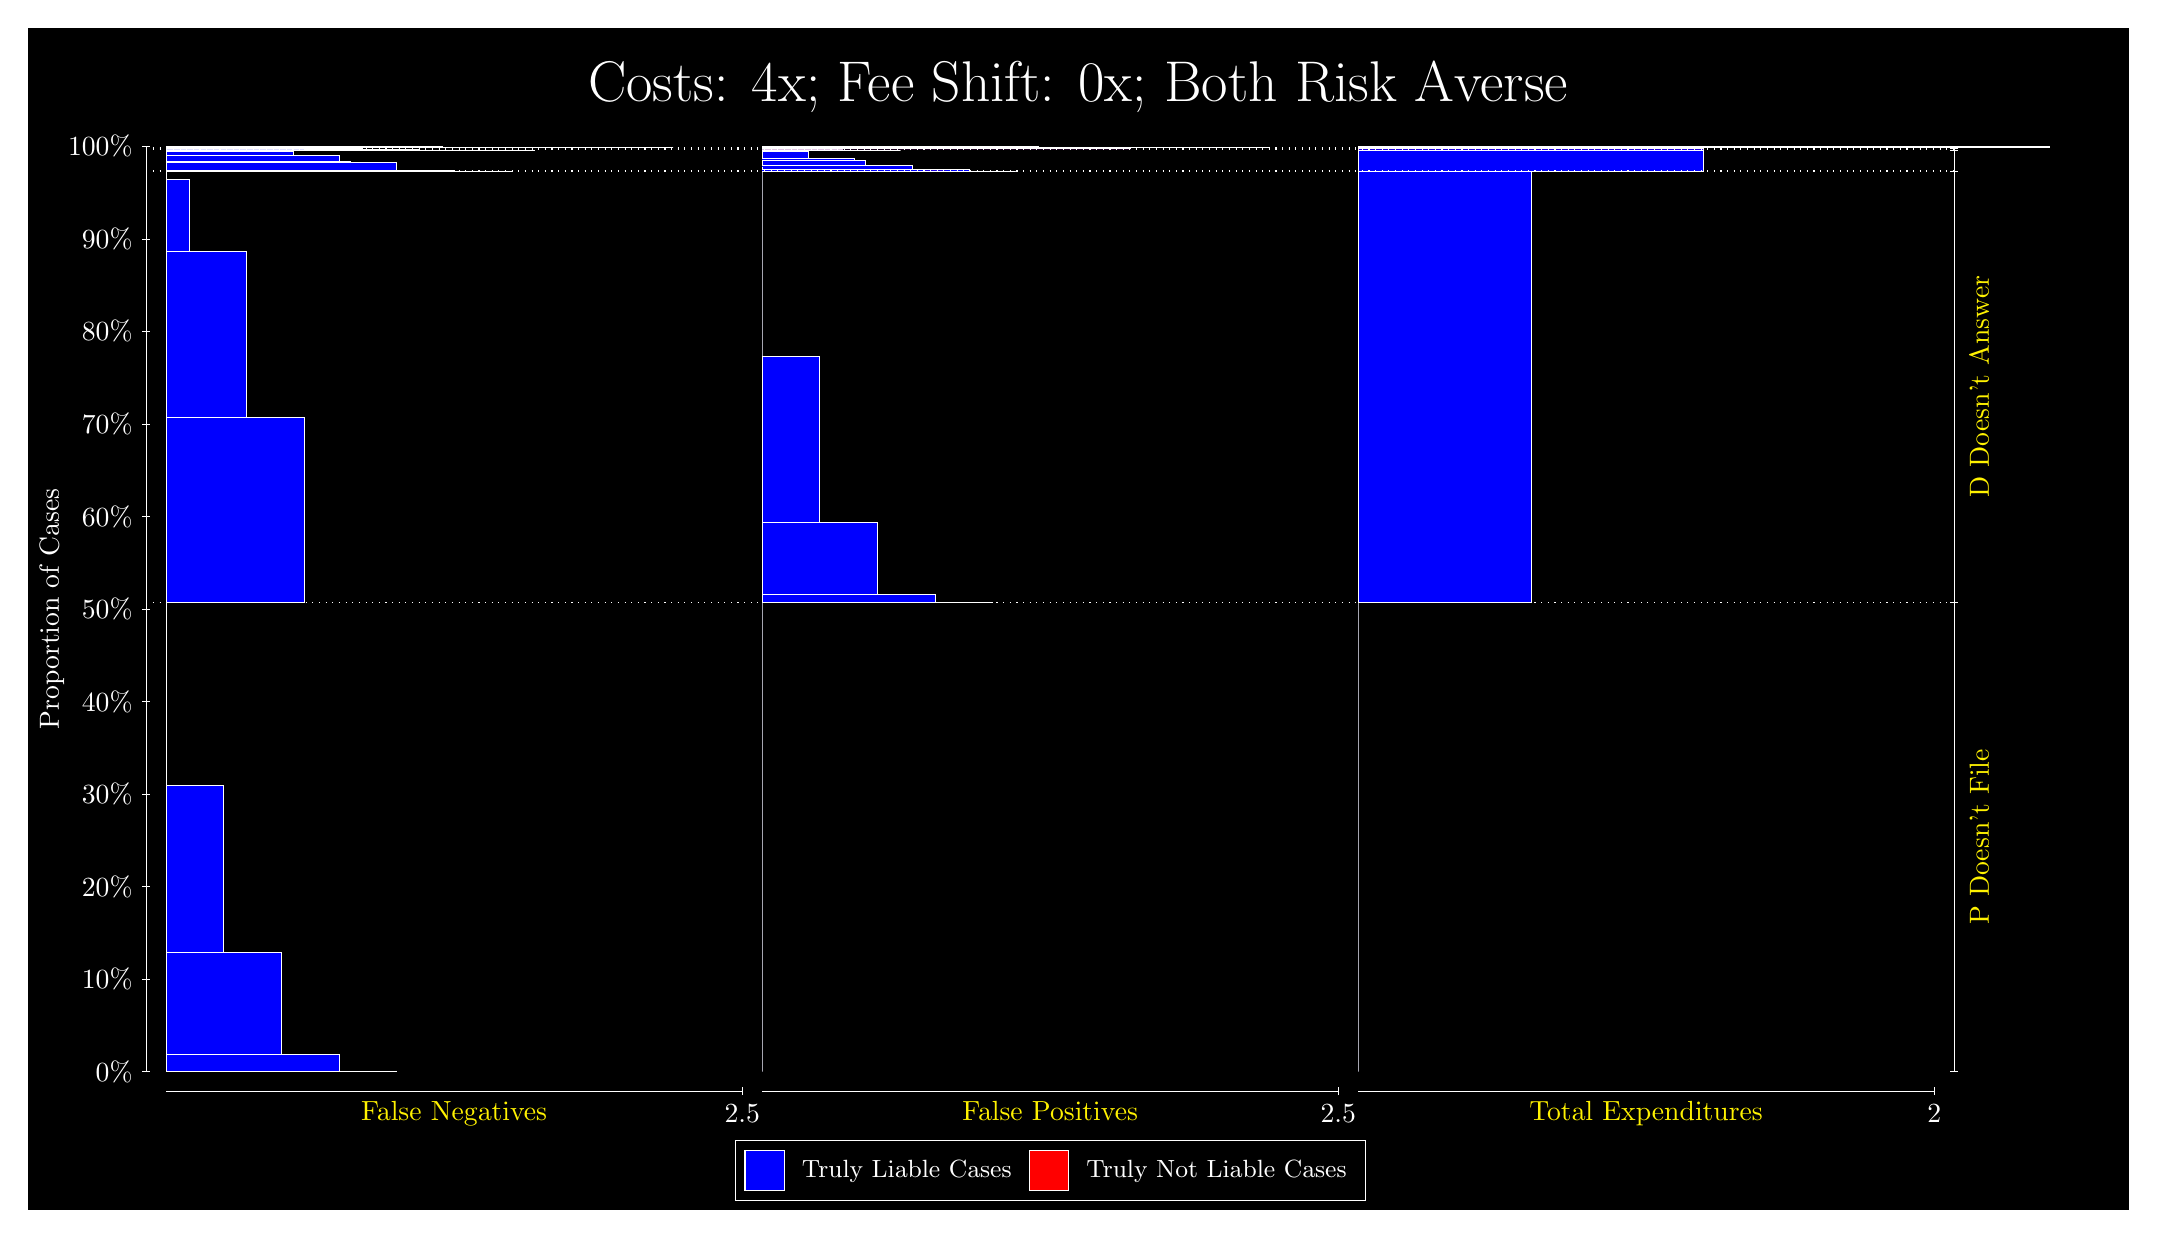
\begin{tikzpicture}
\draw[fill=black] (0,0) rectangle (26.667,15);
\draw[text=white] (0,13.5) rectangle (26.667,15) node[midway] {\huge Costs: 4x; Fee Shift: 0x; Both Risk Averse};
\draw[white, very thin] (1.5,1.75) -- (1.5,13.5);
\node[rotate=90, text=white, anchor=center] at (0.3, 7.625) {Proportion of Cases};
\draw[white, very thin] (1.45,1.75) -- (1.55,1.75);
\node[text=white, anchor=east] at (1.45, 1.75) {0\%};
\draw[white, very thin] (1.45,2.925) -- (1.55,2.925);
\node[text=white, anchor=east] at (1.45, 2.925) {10\%};
\draw[white, very thin] (1.45,4.1) -- (1.55,4.1);
\node[text=white, anchor=east] at (1.45, 4.1) {20\%};
\draw[white, very thin] (1.45,5.275) -- (1.55,5.275);
\node[text=white, anchor=east] at (1.45, 5.275) {30\%};
\draw[white, very thin] (1.45,6.45) -- (1.55,6.45);
\node[text=white, anchor=east] at (1.45, 6.45) {40\%};
\draw[white, very thin] (1.45,7.625) -- (1.55,7.625);
\node[text=white, anchor=east] at (1.45, 7.625) {50\%};
\draw[white, very thin] (1.45,8.8) -- (1.55,8.8);
\node[text=white, anchor=east] at (1.45, 8.8) {60\%};
\draw[white, very thin] (1.45,9.975) -- (1.55,9.975);
\node[text=white, anchor=east] at (1.45, 9.975) {70\%};
\draw[white, very thin] (1.45,11.15) -- (1.55,11.15);
\node[text=white, anchor=east] at (1.45, 11.15) {80\%};
\draw[white, very thin] (1.45,12.325) -- (1.55,12.325);
\node[text=white, anchor=east] at (1.45, 12.325) {90\%};
\draw[white, very thin] (1.45,13.5) -- (1.55,13.5);
\node[text=white, anchor=east] at (1.45, 13.5) {100\%};

\draw[white, very thin] (24.457,1.75) -- (24.457,13.5);
\draw[white, very thin] (24.407,1.75) -- (24.507,1.75);
\node[anchor=west] at (24.407, 1.75) {};
\draw[white, very thin] (24.407,7.7077) -- (24.507,7.7077);
\node[anchor=west] at (24.407, 7.7077) {};
\draw[white, very thin] (24.407,13.186) -- (24.507,13.186);
\node[anchor=west] at (24.407, 13.186) {};
\draw[white, very thin] (24.407,13.455) -- (24.507,13.455);
\node[anchor=west] at (24.407, 13.455) {};
\draw[white, very thin] (24.407,13.472) -- (24.507,13.472);
\node[anchor=west] at (24.407, 13.472) {};
\draw[white, very thin] (24.407,13.49) -- (24.507,13.49);
\node[anchor=west] at (24.407, 13.49) {};
\draw[white, very thin] (24.407,13.5) -- (24.507,13.5);
\node[anchor=west] at (24.407, 13.5) {};

\draw[white, very thin, fill=blue] (1.75,1.75) rectangle (4.6775,1.7522);
\draw[white, very thin, fill=blue] (1.75,1.7522) rectangle (3.9457,1.9712);
\draw[white, very thin, fill=blue] (1.75,1.9712) rectangle (3.2138,3.2626);
\draw[white, very thin, fill=blue] (1.75,3.2626) rectangle (2.4819,5.3799);
\draw[white, very thin, fill=red] (1.75,5.3799) rectangle (1.75,5.3799);
\draw[white, very thin, fill=blue] (1.75,5.3799) rectangle (1.75,7.7077);
\draw[white, very thin, fill=blue] (1.75,7.7077) rectangle (3.5065,10.055);
\draw[white, very thin, fill=blue] (1.75,10.055) rectangle (2.7746,12.165);
\draw[white, very thin, fill=blue] (1.75,12.165) rectangle (2.0428,13.079);
\draw[white, very thin, fill=red] (1.75,13.079) rectangle (1.75,13.079);
\draw[white, very thin, fill=blue] (1.75,13.079) rectangle (1.75,13.186);
\draw[white, very thin, fill=blue] (1.75,13.186) rectangle (6.1413,13.186);
\draw[white, very thin, fill=blue] (1.75,13.186) rectangle (5.8486,13.186);
\draw[white, very thin, fill=blue] (1.75,13.186) rectangle (5.5558,13.186);
\draw[white, very thin, fill=blue] (1.75,13.186) rectangle (5.4094,13.197);
\draw[white, very thin, fill=blue] (1.75,13.197) rectangle (5.1167,13.198);
\draw[white, very thin, fill=blue] (1.75,13.198) rectangle (4.9703,13.198);
\draw[white, very thin, fill=blue] (1.75,13.198) rectangle (4.8239,13.2);
\draw[white, very thin, fill=blue] (1.75,13.2) rectangle (4.6775,13.296);
\draw[white, very thin, fill=blue] (1.75,13.296) rectangle (4.3848,13.297);
\draw[white, very thin, fill=blue] (1.75,13.297) rectangle (4.2384,13.299);
\draw[white, very thin, fill=blue] (1.75,13.299) rectangle (4.092,13.314);
\draw[white, very thin, fill=blue] (1.75,13.314) rectangle (3.9457,13.386);
\draw[white, very thin, fill=blue] (1.75,13.386) rectangle (3.6529,13.386);
\draw[white, very thin, fill=blue] (1.75,13.386) rectangle (3.5065,13.387);
\draw[white, very thin, fill=blue] (1.75,13.387) rectangle (3.3602,13.435);
\draw[white, very thin, fill=blue] (1.75,13.435) rectangle (3.2138,13.436);
\draw[white, very thin, fill=blue] (1.75,13.436) rectangle (2.921,13.436);
\draw[white, very thin, fill=blue] (1.75,13.436) rectangle (2.7746,13.436);
\draw[white, very thin, fill=blue] (1.75,13.436) rectangle (2.6283,13.455);
\draw[white, very thin, fill=blue] (1.75,13.455) rectangle (2.0428,13.455);
\draw[white, very thin, fill=red] (1.75,13.455) rectangle (1.75,13.455);
\draw[white, very thin, fill=blue] (1.75,13.455) rectangle (6.4341,13.455);
\draw[white, very thin, fill=blue] (1.75,13.455) rectangle (5.7022,13.455);
\draw[white, very thin, fill=blue] (1.75,13.455) rectangle (4.9703,13.466);
\draw[white, very thin, fill=blue] (1.75,13.466) rectangle (4.2384,13.472);
\draw[white, very thin, fill=blue] (1.75,13.472) rectangle (3.5065,13.472);
\draw[white, very thin, fill=red] (1.75,13.472) rectangle (1.75,13.472);
\draw[white, very thin, fill=blue] (1.75,13.472) rectangle (3.5065,13.473);
\draw[white, very thin, fill=blue] (1.75,13.473) rectangle (2.7746,13.476);
\draw[white, very thin, fill=blue] (1.75,13.476) rectangle (2.0428,13.488);
\draw[white, very thin, fill=red] (1.75,13.488) rectangle (1.75,13.488);
\draw[white, very thin, fill=blue] (1.75,13.488) rectangle (1.75,13.49);
\draw[white, very thin, fill=blue] (1.75,13.49) rectangle (8.1906,13.49);
\draw[white, very thin, fill=blue] (1.75,13.49) rectangle (7.4587,13.49);
\draw[white, very thin, fill=blue] (1.75,13.49) rectangle (6.7268,13.491);
\draw[white, very thin, fill=blue] (1.75,13.491) rectangle (5.9949,13.493);
\draw[white, very thin, fill=blue] (1.75,13.493) rectangle (5.2631,13.498);
\draw[white, very thin, fill=blue] (1.75,13.498) rectangle (4.5312,13.5);
\draw[white, very thin, fill=blue] (1.75,13.5) rectangle (3.7993,13.5);
\draw[white, very thin, fill=blue] (1.75,13.5) rectangle (3.0674,13.5);
\draw[white, very thin, fill=blue] (1.75,13.5) rectangle (2.3355,13.5);
\draw[white, very thin, fill=red] (1.75,13.5) rectangle (1.75,13.5);
\draw[white, very thin, fill=red] (9.3189,1.75) rectangle (9.3189,1.75);
\draw[white, very thin, fill=blue] (9.3189,1.75) rectangle (9.3189,7.7077);
\draw[white, very thin, fill=red] (9.3189,7.7077) rectangle (12.246,7.7077);
\draw[white, very thin, fill=blue] (9.3189,7.7077) rectangle (12.246,7.7106);
\draw[white, very thin, fill=blue] (9.3189,7.7106) rectangle (11.515,7.8142);
\draw[white, very thin, fill=blue] (9.3189,7.8142) rectangle (10.783,8.7284);
\draw[white, very thin, fill=blue] (9.3189,8.7284) rectangle (10.051,10.838);
\draw[white, very thin, fill=blue] (9.3189,10.838) rectangle (9.3189,13.186);
\draw[white, very thin, fill=red] (9.3189,13.186) rectangle (12.539,13.186);
\draw[white, very thin, fill=blue] (9.3189,13.186) rectangle (12.539,13.186);
\draw[white, very thin, fill=red] (9.3189,13.186) rectangle (11.954,13.186);
\draw[white, very thin, fill=blue] (9.3189,13.186) rectangle (11.954,13.204);
\draw[white, very thin, fill=blue] (9.3189,13.204) rectangle (11.807,13.204);
\draw[white, very thin, fill=red] (9.3189,13.204) rectangle (11.661,13.204);
\draw[white, very thin, fill=blue] (9.3189,13.204) rectangle (11.661,13.204);
\draw[white, very thin, fill=red] (9.3189,13.204) rectangle (11.368,13.204);
\draw[white, very thin, fill=blue] (9.3189,13.204) rectangle (11.368,13.205);
\draw[white, very thin, fill=blue] (9.3189,13.205) rectangle (11.222,13.254);
\draw[white, very thin, fill=blue] (9.3189,13.254) rectangle (11.075,13.255);
\draw[white, very thin, fill=blue] (9.3189,13.255) rectangle (10.929,13.255);
\draw[white, very thin, fill=blue] (9.3189,13.255) rectangle (10.636,13.326);
\draw[white, very thin, fill=blue] (9.3189,13.326) rectangle (10.49,13.342);
\draw[white, very thin, fill=blue] (9.3189,13.342) rectangle (10.344,13.343);
\draw[white, very thin, fill=blue] (9.3189,13.343) rectangle (10.197,13.345);
\draw[white, very thin, fill=blue] (9.3189,13.345) rectangle (9.9044,13.441);
\draw[white, very thin, fill=blue] (9.3189,13.441) rectangle (9.758,13.442);
\draw[white, very thin, fill=blue] (9.3189,13.442) rectangle (9.6116,13.443);
\draw[white, very thin, fill=blue] (9.3189,13.443) rectangle (9.4652,13.444);
\draw[white, very thin, fill=blue] (9.3189,13.444) rectangle (9.3189,13.455);
\draw[white, very thin, fill=red] (9.3189,13.455) rectangle (11.075,13.455);
\draw[white, very thin, fill=blue] (9.3189,13.455) rectangle (11.075,13.455);
\draw[white, very thin, fill=blue] (9.3189,13.455) rectangle (10.344,13.461);
\draw[white, very thin, fill=blue] (9.3189,13.461) rectangle (9.6116,13.472);
\draw[white, very thin, fill=blue] (9.3189,13.472) rectangle (9.3189,13.472);
\draw[white, very thin, fill=red] (9.3189,13.472) rectangle (14.003,13.472);
\draw[white, very thin, fill=blue] (9.3189,13.472) rectangle (14.003,13.472);
\draw[white, very thin, fill=blue] (9.3189,13.472) rectangle (13.271,13.474);
\draw[white, very thin, fill=blue] (9.3189,13.474) rectangle (12.539,13.486);
\draw[white, very thin, fill=blue] (9.3189,13.486) rectangle (11.807,13.49);
\draw[white, very thin, fill=blue] (9.3189,13.49) rectangle (11.075,13.49);
\draw[white, very thin, fill=red] (9.3189,13.49) rectangle (15.759,13.49);
\draw[white, very thin, fill=blue] (9.3189,13.49) rectangle (15.759,13.49);
\draw[white, very thin, fill=blue] (9.3189,13.49) rectangle (15.028,13.49);
\draw[white, very thin, fill=red] (9.3189,13.49) rectangle (15.028,13.49);
\draw[white, very thin, fill=blue] (9.3189,13.49) rectangle (15.028,13.49);
\draw[white, very thin, fill=blue] (9.3189,13.49) rectangle (14.296,13.491);
\draw[white, very thin, fill=red] (9.3189,13.491) rectangle (14.296,13.491);
\draw[white, very thin, fill=blue] (9.3189,13.491) rectangle (14.296,13.491);
\draw[white, very thin, fill=blue] (9.3189,13.491) rectangle (13.564,13.491);
\draw[white, very thin, fill=red] (9.3189,13.491) rectangle (13.564,13.491);
\draw[white, very thin, fill=blue] (9.3189,13.491) rectangle (13.564,13.493);
\draw[white, very thin, fill=blue] (9.3189,13.493) rectangle (12.832,13.493);
\draw[white, very thin, fill=red] (9.3189,13.493) rectangle (12.832,13.493);
\draw[white, very thin, fill=blue] (9.3189,13.493) rectangle (12.832,13.498);
\draw[white, very thin, fill=blue] (9.3189,13.498) rectangle (12.1,13.5);
\draw[white, very thin, fill=blue] (9.3189,13.5) rectangle (11.368,13.5);
\draw[white, very thin, fill=blue] (9.3189,13.5) rectangle (10.636,13.5);
\draw[white, very thin, fill=blue] (9.3189,13.5) rectangle (9.9044,13.5);
\draw[white, very thin, fill=red] (16.888,1.75) rectangle (16.888,1.75);
\draw[white, very thin, fill=blue] (16.888,1.75) rectangle (16.888,7.7077);
\draw[white, very thin, fill=red] (16.888,7.7077) rectangle (19.083,7.7077);
\draw[white, very thin, fill=blue] (16.888,7.7077) rectangle (19.083,13.186);
\draw[white, very thin, fill=red] (16.888,13.186) rectangle (21.279,13.186);
\draw[white, very thin, fill=blue] (16.888,13.186) rectangle (21.279,13.189);
\draw[white, very thin, fill=red] (16.888,13.189) rectangle (21.279,13.189);
\draw[white, very thin, fill=blue] (16.888,13.189) rectangle (21.279,13.455);
\draw[white, very thin, fill=red] (16.888,13.455) rectangle (21.279,13.455);
\draw[white, very thin, fill=blue] (16.888,13.455) rectangle (21.279,13.472);
\draw[white, very thin, fill=red] (16.888,13.472) rectangle (21.279,13.472);
\draw[white, very thin, fill=blue] (16.888,13.472) rectangle (21.279,13.49);
\draw[white, very thin, fill=red] (16.888,13.49) rectangle (25.67,13.49);
\draw[white, very thin, fill=blue] (16.888,13.49) rectangle (25.67,13.491);
\draw[white, very thin, fill=red] (16.888,13.491) rectangle (25.67,13.491);
\draw[white, very thin, fill=blue] (16.888,13.491) rectangle (25.67,13.5);
\draw[white, dotted] (1.5,7.7077) -- (24.457,7.7077);
\draw[white, dotted] (1.5,13.186) -- (24.457,13.186);
\draw[white, dotted] (1.5,13.455) -- (24.457,13.455);
\draw[white, dotted] (1.5,13.472) -- (24.457,13.472);
\draw[white, dotted] (1.5,13.49) -- (24.457,13.49);
\draw[white, very thin] (1.75,1.5) -- (9.0689,1.5);
\node[text=yellow, anchor=north] at (5.4094, 1.5) {False Negatives};
\draw[white, very thin] (9.0689,1.45) -- (9.0689,1.55);
\node[text=white, anchor=north] at (9.0689, 1.45) {2.5};

\draw[white, very thin] (9.3189,1.5) -- (16.638,1.5);
\node[text=yellow, anchor=north] at (12.978, 1.5) {False Positives};
\draw[white, very thin] (16.638,1.45) -- (16.638,1.55);
\node[text=white, anchor=north] at (16.638, 1.45) {2.5};

\draw[white, very thin] (16.888,1.5) -- (24.207,1.5);
\node[text=yellow, anchor=north] at (20.547, 1.5) {Total Expenditures};
\draw[white, very thin] (24.207,1.45) -- (24.207,1.55);
\node[text=white, anchor=north] at (24.207, 1.45) {2};

\node[text=yellow, centered, rotate=90] at (24.777, 4.7289) {P Doesn't File};
\node[text=yellow, centered, rotate=90] at (24.777, 10.447) {D Doesn't Answer};





\draw (12.978300999999998,1.5) node[draw=none] (baseCoordinate) {};
\begin{scope}[align=center]
        \matrix[scale=0.5, draw=white, below=0.5cm of baseCoordinate, nodes={draw}, column sep=0.1cm]{
            \node[rectangle, draw, minimum width=0.5cm, minimum height=0.5cm, fill=blue] {}; &
            \node[draw=none, font=\small, text=white] (B) {Truly Liable Cases}; &
            \node[rectangle, draw, minimum width=0.5cm, minimum height=0.5cm, fill=red] {}; &
            \node[draw=none, font=\small, text=white] (B) {Truly Not Liable Cases}; \\
            };
\end{scope}

\end{tikzpicture}
\end{document}